\documentclass{ximera}

 

\usepackage{epsfig}

\graphicspath{
  {./}
  {figures/}
}

\usepackage{morewrites}
\makeatletter
\newcommand\subfile[1]{%
\renewcommand{\input}[1]{}%
\begingroup\skip@preamble\otherinput{#1}\endgroup\par\vspace{\topsep}
\let\input\otherinput}
\makeatother

\newcommand{\includeexercises}{\directlua{dofile("/home/jim/linearAlgebra/laode/exercises.lua")}}

%\newcounter{ccounter}
%\setcounter{ccounter}{1}
%\newcommand{\Chapter}[1]{\setcounter{chapter}{\arabic{ccounter}}\chapter{#1}\addtocounter{ccounter}{1}}

%\newcommand{\section}[1]{\section{#1}\setcounter{thm}{0}\setcounter{equation}{0}}

%\renewcommand{\theequation}{\arabic{chapter}.\arabic{section}.\arabic{equation}}
%\renewcommand{\thefigure}{\arabic{chapter}.\arabic{figure}}
%\renewcommand{\thetable}{\arabic{chapter}.\arabic{table}}

%\newcommand{\Sec}[2]{\section{#1}\markright{\arabic{ccounter}.\arabic{section}.#2}\setcounter{equation}{0}\setcounter{thm}{0}\setcounter{figure}{0}}

\newcommand{\Sec}[2]{\section{#1}}

\setcounter{secnumdepth}{2}
%\setcounter{secnumdepth}{1} 

%\newcounter{THM}
%\renewcommand{\theTHM}{\arabic{chapter}.\arabic{section}}

\newcommand{\trademark}{{R\!\!\!\!\!\bigcirc}}
%\newtheorem{exercise}{}

\newcommand{\dfield}{{\sf dfield9}}
\newcommand{\pplane}{{\sf pplane9}}

\newcommand{\EXER}{\section*{Exercises}}%\vspace*{0.2in}\hrule\small\setcounter{exercise}{0}}
\newcommand{\CEXER}{}%\vspace{0.08in}\begin{center}Computer Exercises\end{center}}
\newcommand{\TEXER}{} %\vspace{0.08in}\begin{center}Hand Exercises\end{center}}
\newcommand{\AEXER}{} %\vspace{0.08in}\begin{center}Hand Exercises\end{center}}

% BADBAD: \newcommand{\Bbb}{\bf}

\newcommand{\R}{\mbox{$\Bbb{R}$}}
\newcommand{\C}{\mbox{$\Bbb{C}$}}
\newcommand{\Z}{\mbox{$\Bbb{Z}$}}
\newcommand{\N}{\mbox{$\Bbb{N}$}}
\newcommand{\D}{\mbox{{\bf D}}}
\usepackage{amssymb}
%\newcommand{\qed}{\hfill\mbox{\raggedright$\square$} \vspace{1ex}}
%\newcommand{\proof}{\noindent {\bf Proof:} \hspace{0.1in}}

\newcommand{\setmin}{\;\mbox{--}\;}
\newcommand{\Matlab}{{M\small{AT\-LAB}} }
\newcommand{\Matlabp}{{M\small{AT\-LAB}}}
\newcommand{\computer}{\Matlab Instructions}
\newcommand{\half}{\mbox{$\frac{1}{2}$}}
\newcommand{\compose}{\raisebox{.15ex}{\mbox{{\scriptsize$\circ$}}}}
\newcommand{\AND}{\quad\mbox{and}\quad}
\newcommand{\vect}[2]{\left(\begin{array}{c} #1_1 \\ \vdots \\
 #1_{#2}\end{array}\right)}
\newcommand{\mattwo}[4]{\left(\begin{array}{rr} #1 & #2\\ #3
&#4\end{array}\right)}
\newcommand{\mattwoc}[4]{\left(\begin{array}{cc} #1 & #2\\ #3
&#4\end{array}\right)}
\newcommand{\vectwo}[2]{\left(\begin{array}{r} #1 \\ #2\end{array}\right)}
\newcommand{\vectwoc}[2]{\left(\begin{array}{c} #1 \\ #2\end{array}\right)}

\newcommand{\ignore}[1]{}


\newcommand{\inv}{^{-1}}
\newcommand{\CC}{{\cal C}}
\newcommand{\CCone}{\CC^1}
\newcommand{\Span}{{\rm span}}
\newcommand{\rank}{{\rm rank}}
\newcommand{\trace}{{\rm tr}}
\newcommand{\RE}{{\rm Re}}
\newcommand{\IM}{{\rm Im}}
\newcommand{\nulls}{{\rm null\;space}}

\newcommand{\dps}{\displaystyle}
\newcommand{\arraystart}{\renewcommand{\arraystretch}{1.8}}
\newcommand{\arrayfinish}{\renewcommand{\arraystretch}{1.2}}
\newcommand{\Start}[1]{\vspace{0.08in}\noindent {\bf Section~\ref{#1}}}
\newcommand{\exer}[1]{\noindent {\bf \ref{#1}}}
\newcommand{\ans}{}
\newcommand{\matthree}[9]{\left(\begin{array}{rrr} #1 & #2 & #3 \\ #4 & #5 & #6
\\ #7 & #8 & #9\end{array}\right)}
\newcommand{\cvectwo}[2]{\left(\begin{array}{c} #1 \\ #2\end{array}\right)}
\newcommand{\cmatthree}[9]{\left(\begin{array}{ccc} #1 & #2 & #3 \\ #4 & #5 &
#6 \\ #7 & #8 & #9\end{array}\right)}
\newcommand{\vecthree}[3]{\left(\begin{array}{r} #1 \\ #2 \\
#3\end{array}\right)}
\newcommand{\cvecthree}[3]{\left(\begin{array}{c} #1 \\ #2 \\
#3\end{array}\right)}
\newcommand{\cmattwo}[4]{\left(\begin{array}{cc} #1 & #2\\ #3
&#4\end{array}\right)}

\newcommand{\Matrix}[1]{\ensuremath{\left(\begin{array}{rrrrrrrrrrrrrrrrrr} #1 \end{array}\right)}}

\newcommand{\Matrixc}[1]{\ensuremath{\left(\begin{array}{cccccccccccc} #1 \end{array}\right)}}



\renewcommand{\labelenumi}{\theenumi)}
\newenvironment{enumeratea}%
{\begingroup
 \renewcommand{\theenumi}{\alph{enumi}}
 \renewcommand{\labelenumi}{(\theenumi)}
 \begin{enumerate}}
 {\end{enumerate}\endgroup}



\newcounter{help}
\renewcommand{\thehelp}{\thesection.\arabic{equation}}

%\newenvironment{equation*}%
%{\renewcommand\endequation{\eqno (\theequation)* $$}%
%   \begin{equation}}%
%   {\end{equation}\renewcommand\endequation{\eqno \@eqnnum
%$$\global\@ignoretrue}}

%\input{psfig.tex}

\author{Martin Golubitsky and Michael Dellnitz}

%\newenvironment{matlabEquation}%
%{\renewcommand\endequation{\eqno (\theequation*) $$}%
%   \begin{equation}}%
%   {\end{equation}\renewcommand\endequation{\eqno \@eqnnum
% $$\global\@ignoretrue}}

\newcommand{\soln}{\textbf{Solution:} }
\newcommand{\exercap}[1]{\centerline{Figure~\ref{#1}}}
\newcommand{\exercaptwo}[1]{\centerline{Figure~\ref{#1}a\hspace{2.1in}
Figure~\ref{#1}b}}
\newcommand{\exercapthree}[1]{\centerline{Figure~\ref{#1}a\hspace{1.2in}
Figure~\ref{#1}b\hspace{1.2in}Figure~\ref{#1}c}}
\newcommand{\para}{\hspace{0.4in}}

\renewenvironment{solution}{\suppress}{\endsuppress}

\ifxake
\newenvironment{matlabEquation}{\begin{equation}}{\end{equation}}
\else
\newenvironment{matlabEquation}%
{\let\oldtheequation\theequation\renewcommand{\theequation}{\oldtheequation*}\begin{equation}}%
  {\end{equation}\let\theequation\oldtheequation}
\fi

\makeatother


\title{Chaos and the Lorenz Equation}

\begin{document}
\begin{abstract}
\end{abstract}
\maketitle


\label{S:chaos} \index{chaos}\index{Lorenz system}


Classifying all of the kinds of solutions that can occur asymptotically in 
autonomous systems of first order differential equations is a difficult task 
and is very much a topic of current research.  Until now we have discussed 
three types of solutions: equilibria, limit cycles, and quasiperiodic
motions.  The purpose of the next example, the Lorenz equations, is to 
illustrate that there are still other types of asymptotic behavior that can 
occur in solutions to autonomous ordinary differential equations in three 
dimensions.  This type of solution is called {\em chaotic\/} and what 
distinguishes chaotic solutions from the previously discussed solutions is 
{\em sensitive dependence on initial conditions\/}. \index{chaos}

The prototypical example of chaos is the {\em Lorenz system}. 
\index{Lorenz system}  The Lorenz system consists of three first order 
(almost linear) ordinary differential equations (there are just two quadratic 
terms):
\begin{matlabEquation}  \label{e:Lorenz}
\begin{array}{rcl}
\dot{x}_1 & = & \sigma(x_2-x_1)\\
\dot{x}_2 & = & \rho x_1 - x_2 - x_1x_3\\
\dot{x}_3 & = & -\beta x_3 + x_1x_2,
\end{array}
\end{matlabEquation}
where $\sigma$, $\rho$ and $\beta$ are real constants.  We consider here
solutions to \eqref{e:Lorenz} when
\[
\sigma=10,\quad \beta=\frac{8}{3},\quad \rho=28.
\]
The right hand side of \eqref{e:Lorenz} is stored in the m-file {\tt f14\_6\_1.m}:
\begin{verbatim}
function f = f14_6_1(t,x)
sigma = 10;  beta  = 8/3;  rho   = 28;
f     = [sigma*(x(2)-x(1));
         rho*x(1)-x(2)-x(1)*x(3);
         -beta*x(3)+x(1)*x(2)];
\end{verbatim}

\begin{figure}[bht]
   \centerline{%
   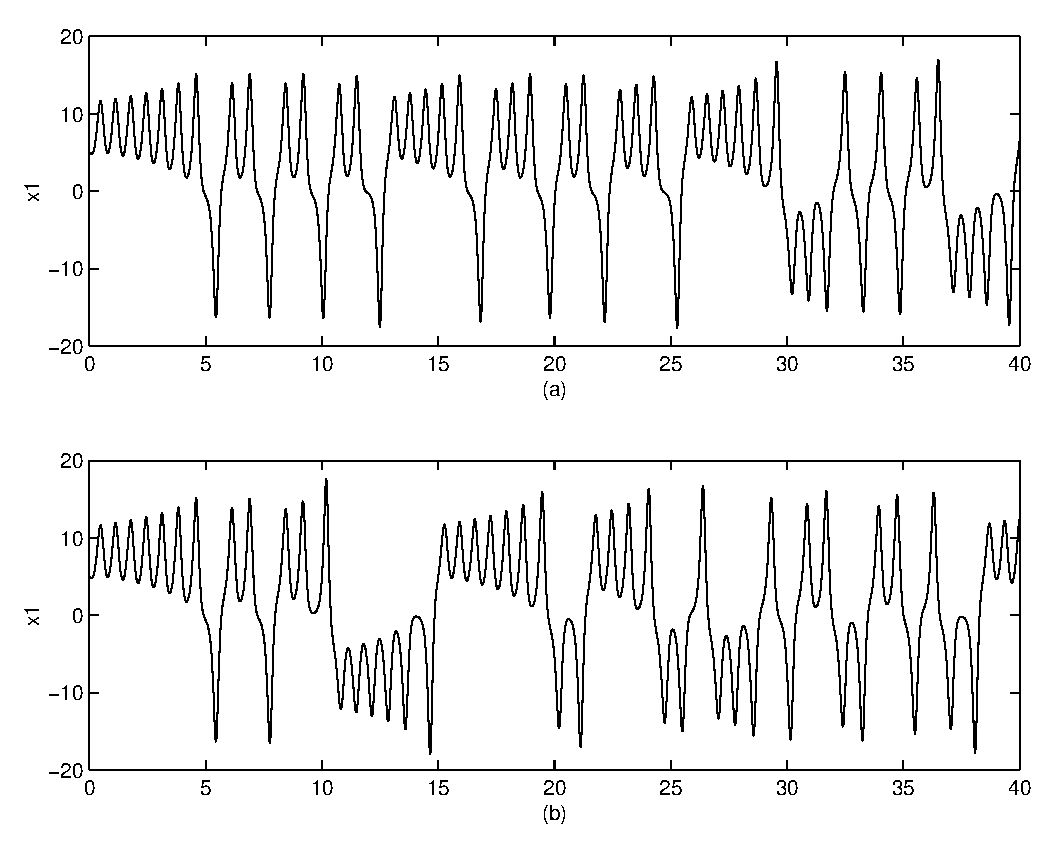
\psfig{file=../figures/lorenz12.eps,width=3.0in}}
   \caption{Approximation of chaotic solutions of the Lorenz system by 
	{\tt ode45} illustrating sensitive dependence on initial conditions.  
	(a) A solution starting at $(5,5,30)$;  (b) a solution starting at 
	$(5.01,5,30)$.}
   \label{fig:lorenz1}
\end{figure}

Compute a solution of the Lorenz system\index{Lorenz system} starting at 
$X_0=(5,5,30)$ by typing
\begin{verbatim}
[t,x]=ode45('f14_6_1',[0 40],[5,5,30]');
\end{verbatim}
The time series of $x_1$ is shown in Figure~\ref{fig:lorenz1}(a).  This time 
series looks bizarre and no apparent regularity can be seen.  Moreover, the 
motion is not just irregular, it is also sensitive to the choice of the initial 
conditions.  \index{sensitivity to initial conditions}


\subsubsection*{Sensitive Dependence on Initial Conditions}

In Figure~\ref{fig:lorenz1}(b) we illustrate sensitive dependence by showing  
a solution of the Lorenz system\index{Lorenz system} with initial conditions 
very close to the first one, namely at $X_0=(5.01,5,30)$.  In the beginning 
the solutions behave in a similar way, but by $t\approx 10$ the behavior is 
completely different.  Even for smaller 
differences in the initial conditions, the phenomenon of sensitivity to 
initial conditions is still present, although the significant difference in 
the trajectories occurs at a later time (see Figure~\ref{fig:lorenz2}).  

\begin{figure}[htb]
   \centerline{%
   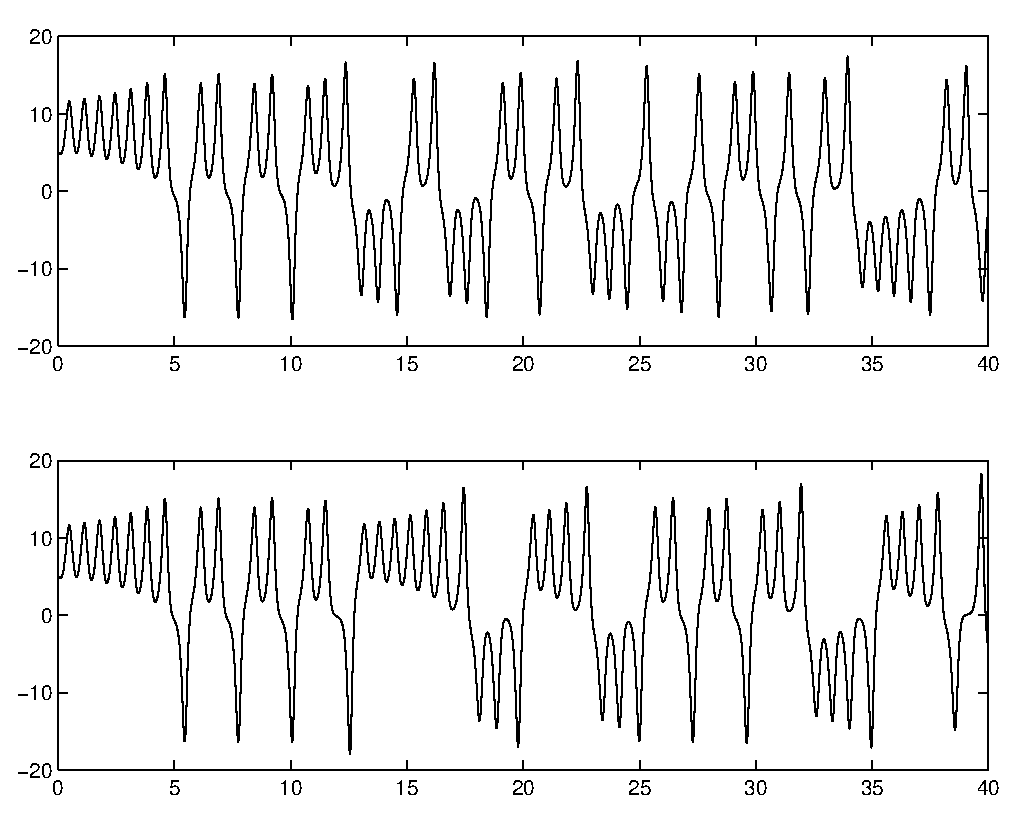
\psfig{file=../figures/lorenz34.eps,width=3.0in}}
   \caption{Approximation of chaotic solutions of the Lorenz system by 
	{\tt ode45} illustrating sensitive dependence on initial conditions.
 	 (a) A solution starting at $(5.001,5,30)$;
  	 (b) a solution starting at $(5.0001,5,30)$.}
   \label{fig:lorenz2}
\end{figure}

The consequence of sensitive dependence of solutions on initial conditions in 
the Lorenz system is in long term unpredictable behavior.  Typically, in
experiments, we know initial conditions only to within some (hopefully) small
error.  If these errors get magnified, as they do in the Lorenz system, then
it is impossible to make accurate long term predictions.  This lack of
predictability is the defining feature of {\em chaotic behavior}.
\index{chaos}  So we must ask:  Is chaotic behavior typical in solutions to
autonomous systems of differential equations?  The answer is yes.  Not every
three dimensional systems of differential equations exhibits chaos --- but
many do.  

In Figure~\ref{fig:lorenz3} we show a phase space plot of the
solution starting at $(5,5,30)$.  To reproduce this figure with the 
correct scale and view point type
\begin{verbatim}
[t,x]=ode45('f14_6_1',[0 40],[5,5,30]');
plot3(x(:,1),x(:,2),x(:,3))
axis([-20,20,-20,20,0,60])
view(125,20)
\end{verbatim}\index{\computer!plot3}\index{\computer!axis}\index{\computer!view}
\begin{figure}[htb]
   \centerline{%
   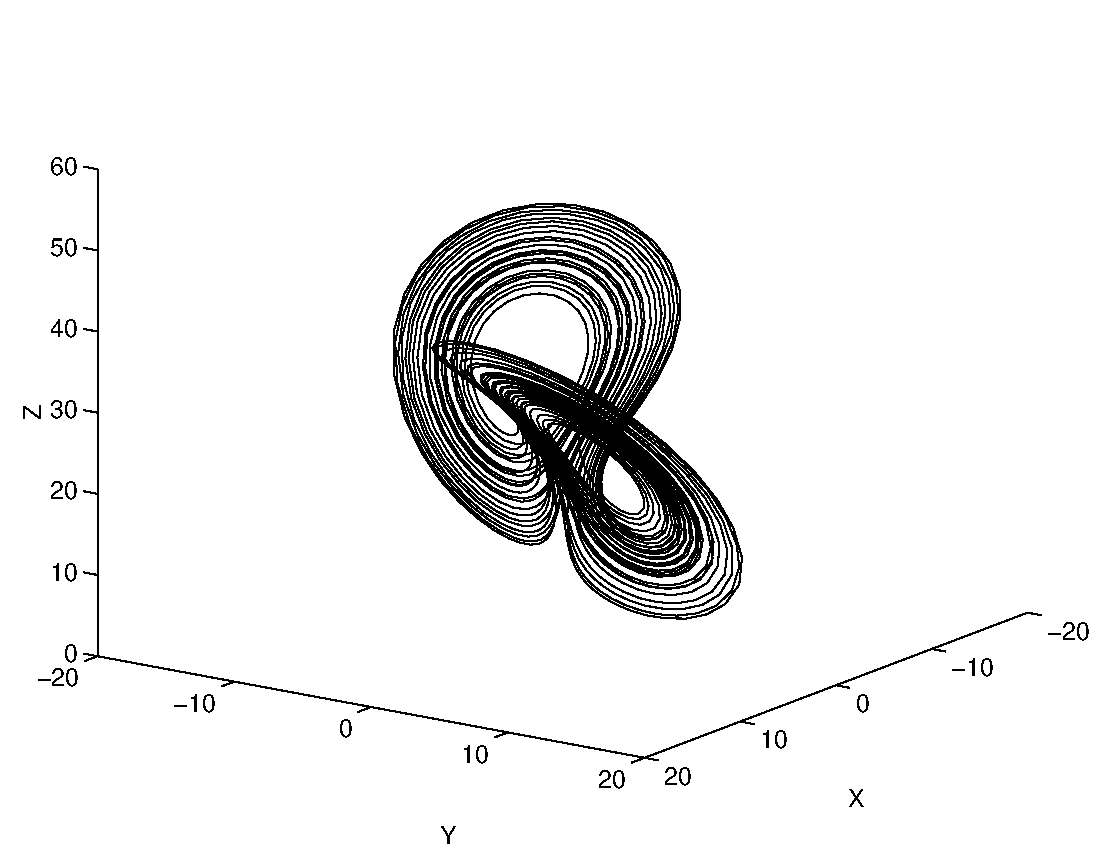
\psfig{file=../figures/lorenz5.eps,width=5.5in}}
   \caption{Phase space plot of a solution of the Lorenz system
   starting at $(5,5,30)$.}
   \label{fig:lorenz3}
\end{figure}

We emphasize that the existence of sensitive dependence on initial conditions 
does {\em not\/} depend on the numerical algorithm used in the numerical 
integration nor does it depend on the computer that is used.  However, 
different numerical algorithms and even different computers will give 
different numerical results.   Finally, we note that the phase space picture 
of the Lorenz attractor\index{Lorenz attractor}, as shown in 
Figure~\ref{fig:lorenz3}, will seem the same to the eye, independent of the 
choice of numerical algorithm and computer,
even though the time series will have readily observable differences of the
type shown in Figure~\ref{fig:lorenz2}.  {\bf Remark:}  A dynamic simulation 
of a solution to the Lorenz equations in phase space can also be seen in 
\Matlabp: just type {\tt lorenz}.\index{\computer!lorenz}

It should be noted that even though quasiperiodic motion is geometrically 
complicated (leading to trajectories lying on a torus), it does not exhibit
sensitive dependence on initial conditions.  More precisely, the time series 
of asymptotically stable quasiperiodic solutions remain almost unchanged 
after small changes in initial conditions.  To verify this statement, we 
return to the numerical solution of \eqref{e:ftor3}.  In Figure~\ref{F:tor3tsab}
we plot the time series for the $x_1$ component of solutions with nearly 
identical initial conditions and note that the two time series are nearly 
identical.

\begin{figure}[htb]
   \centerline{%
   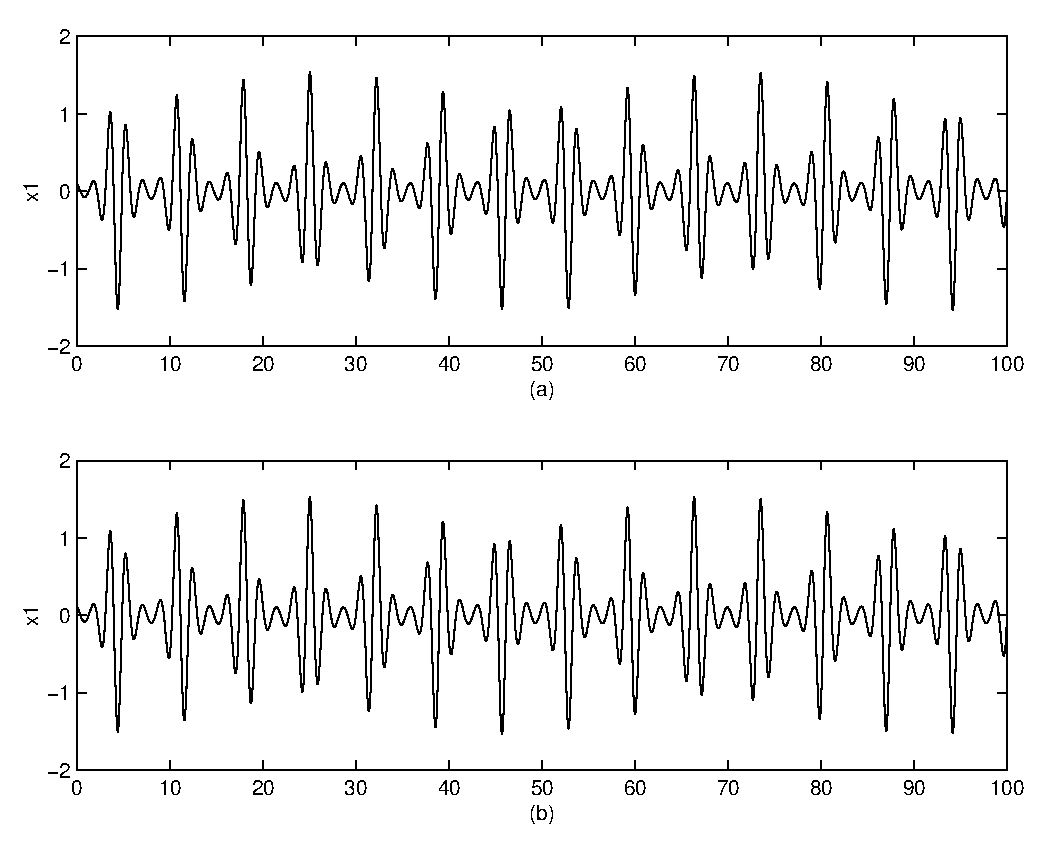
\psfig{file=../figures/ftor3tsab.eps,width=3.0in}}
   \caption{Time series for a quasiperiodic two-frequency solution of the 
	nonlinear system \protect\eqref{e:ftor3} illustrating a lack of sensitive 
	dependence on initial conditions: (a) $X_0=(0.1,0.03,0.001)$ and (b) 
	$X_0=(0.11,0.031,0.0015)$.}
   \label{F:tor3tsab}
\end{figure}

\subsection*{A Summary of Observed Three-Dimensional Dynamics}

We now summarize the types of attracting solutions that we have seen in
autonomous three-dimensional systems of differential equations.  The states
we have studied are stable equilibria (or sinks), attracting limit cycles,
attracting quasiperiodic two-frequency motions, and chaotic dynamics such as
seen in the Lorenz equations.  Each of these solution types has well-defined
characteristics that can be observed either in time series plots or in
three-dimensional phase space plots.  This information is summarized in 
Table~\ref{T:assdyn}.

\begin{table}
\begin{center}
\begin{tabular}{|c|c|c|}
\hline
\begin{minipage}[t]{1.1in}
\begin{center}
Asymptotic \\
Solution Type 
\end{center}
\end{minipage}
& Times Series & Phase Space \\
\hline
\hline
sink 
&
horizontal line
&
point \\
\hline
limit cycle
&
periodic oscillation 
&
`circle'
\\ \hline
\begin{minipage}[t]{1.0in}
\begin{center}
two-frequency \\
quasiperiodic 
\end{center}
\end{minipage}
& 
modulated periodic oscillation 
& 
torus
\\ \hline
chaotic 
&
\begin{minipage}[t]{2.3in}
\begin{center}
bounded irregular oscillation \\ 
{\bf with} sensitive dependence \\
on initial conditions
\end{center}
\end{minipage}
&
\begin{minipage}[t]{1.7in}
\begin{center}
complicated surface \\
{\bf not} sensitive \\
to initial conditions
\end{center}
\end{minipage}
\\ \hline
\end{tabular}
\end{center}
\caption{Summary of Observed Asymptotic Dynamics in Three Dimensions}
\label{T:assdyn}
\end{table} 

In Figure~\ref{fig:flinear1} we plotted the time series of a solution to a 
linear equation $\dot{X}=AX$ where the $3\times 3$ matrix $A$ had eigenvalues
with negative real part.  These time series showed convergence to the 
equilibrium at the origin by becoming horizontal as $t$ increased.  There was
transient oscillation caused by a complex conjugate pair of eigenvalues in 
$A$.  The three-dimensional phase portrait Figure~\ref{fig:flinear2} indicates
convergence of this solution trajectory to a point.  These types of time 
series and phase portraits are equally valid for nonlinear systems near a sink,
as was illustrated in Figure~\ref{F:fnonlin3} for the nonlinear system \eqref{E:fnonlin}.

In example \eqref{E:3per}, we saw a solution to an autonomous three-dimensional 
system of differential equations approach a limit cycle.  For such 
examples, the time series converge to a periodic function, as in 
Figure~\ref{F:3per}.  In phase space, such solutions converge to a closed 
curve, like a circle.  See Figure~\ref{F:3perps}.   In general, the closed 
curve corresponding to a periodic solution can be quite complicated --- but 
the time series will still consist of periodic functions.

The time series for two-frequency quasiperiodic solutions was illustrated for
a four-dimensional linear system in Figure~\ref{F:ftor4ts}.  Note the `almost 
periodic' behavior on short time scales coupled with long time modulations.
The short period oscillation is caused by the larger frequency and the long 
time modulation by the smaller frequency.  Such solutions are found in linear 
systems when there are two complex conjugate pairs of purely imaginary 
eigenvalues with incommensurate frequencies.  Therefore, two-frequency 
motions can only appear in linear systems with four or more variables.  
However, two-frequency quasiperiodic motion can occur in three-dimensional 
nonlinear systems, as illustrated in the time series plots of \eqref{e:ftor3} 
given in Figure~\ref{F:tor3ts}.  In phase space the images are even more 
interesting as, after an initial transient, the solution fills out the 
surface of a torus.  See Figure~\ref{F:tor3ps}.

The Lorenz system \eqref{e:Lorenz} illustrates the possibility of yet more 
complicated motions occurring in three dimensions.  The time series in 
Figures~\ref{fig:lorenz1} and \ref{fig:lorenz2} illustrate the phenomenon of 
sensitive dependence on initial conditions, where the numerical values of 
solutions starting at two nearby initial conditions seem to be unrelated 
after numerically integrating the equations for a relatively short length of 
time.  Nevertheless, the characteristic three-dimensional phase space picture 
of the Lorenz equations shown in Figure~\ref{fig:lorenz3} is reproduced by 
almost all nearby initial conditions.  See Exercise~\ref{c11.4.3a}.
 
Other types of solutions are possible in three dimensions.  Such solutions
are not regular in the sense that they limit on a point, a circle, or a
torus, and they do not exhibit sensitive dependence on initial conditions.  
Although the existence of these other solutions is quite an interesting
topic, we will not pursue it here. 


\EXER

\CEXER



\begin{exercise} \label{c11.4.1}
Compute the three equilibria of the Lorenz system \eqref{e:Lorenz}
\index{Lorenz system!equilibria}
and use {\tt ode45} to decide whether or not these are stable.

\begin{solution}
\ans The system has unstable equilibria $X_1 = (0,0,0)$, 
$X_2 = (6\sqrt{2},6\sqrt{2},27)$, and $X_3 = (-6\sqrt{2},-6\sqrt{2},27)$.

\soln The equilibria of the system occur when $\dot{x_1} = 0$, $\dot{x_2}
= 0$, and $\dot{x_3} = 0$.  According to the first equation of the Lorenz
system, $\dot{x_1} = 0$ when $x_1 = x_2$.  Thus, at the equilibria, the
other two equations can be rewritten
\[
\begin{array}{rcl}
0 & = & \dot{x_2} = \rho x_1 - x_1 - x_1x_3 = x_1(\rho - 1 - x_3). \\
0 & = & \dot{x_3} = -\beta x_3 + x_1^2. \\
\end{array}
\]
So, the system is in equilibrium either at the origin, $X =
(\sqrt{\beta (\rho - 1)}, \sqrt{\beta (\rho - 1)}, \rho 1)$, or
$X = (-\sqrt{\beta (\rho - 1)}, -\sqrt{\beta (\rho - 1)}, \rho - 1)$.
To compute the stabilities at the equilibria, first find the general
Jacobian matrix for the system:
\[
dJ = \cmatthree{-\sigma}{\sigma}{0}{\rho - x_3}{-1}{-x_1}{x_2}{x_1}{-\beta}.
\]
Substitute in the values $\beta = -\frac{8}{3}$, $\rho = 28$, and $\sigma
= 10$ to obtain
\[
dJ = \cmatthree{-10}{10}{0}{28 - x_3}{-1}{-x_1}{x_2}{x_1}{-\frac{8}{3}}
\]
and $X_1 = (0,0,0)$, $X_2 = (6\sqrt{2},6\sqrt{2},27)$, and
$X_3 = (-6\sqrt{2},-6\sqrt{2},27)$.  Then compute the eigenvalues at the
equilibria.  At $X_1$, there are two negative real eigenvalues and one 
positive real eigenvalue, so $X_1$ cannot be stable.  At $X_2$ and $X_3$,
there is one negative real eigenvalue and a pair of complex conjugate
eigenvalues with positive real part.  Determine numerically that most
initial conditions do not converge on either $X_2$ or $X_3$ in forward time,
so $X_2$ and $X_3$ are not stable.


\end{solution}
\end{exercise}

\begin{exercise} \label{c11.4.2}
Fix the parameters $\sigma=10$ and $\beta = 8/3$.  Then
use {\tt ode45} to investigate the behavior of the Lorenz system
\eqref{e:Lorenz} for $\rho=0.8$, $\rho=6$, $\rho=20$ and $\rho=26$.

\begin{solution}

At $\rho = 0.8$, $X_2$ and $X_3$ do not exist, so there is only one
equilibrium $X_1 = (0,0,0)$, which is asymptotically stable.  Thus, all
initial conditions approach the origin in forward time.

\para At $\rho = 6$, there exist equilibria at $X_1 = (0,0,0)$, $X_2 =
(2\sqrt{\frac{10}{3}}, 2\sqrt{\frac{10}{3}}, 5)$, and
$X_3 = (-2\sqrt{\frac{10}{3}}, -2\sqrt{\frac{10}{3}}, 5)$.  All solutions
approach $X_2$ in forward time, so $X_2$ is a stable equilibrium.

\para At $\rho = 20$, all solutions approach $X_3 = (-4\sqrt{\frac{10}{3}},
-4\sqrt{\frac{10}{3}}, 19)$, which is a stable equilibrium.

\para At $\rho = 26$, there is no stable equilibrium.  There are a few
stable trajectories corresponding to negative eigenvalues of the Jacobian
matrices at the equilibria.  For instance, at $X_1 = (0,0,0)$, the Jacobian
has an eigenvalue $\lambda = -\frac{8}{3}$ with eigenvector $v = (0,0,1)$.
The trajectory with initial condition $v$ approaches the origin in forward
time.

\para Figures~\ref{c11.4.2}a -- \ref{c11.4.2}d show the system with
initial condition $X_0 = (5,5,30)$ and $\rho = 0.8$, $\rho = 6$, $\rho = 20$,
and $\rho = 26$.

\begin{figure}[htb]
                       \centerline{%
                       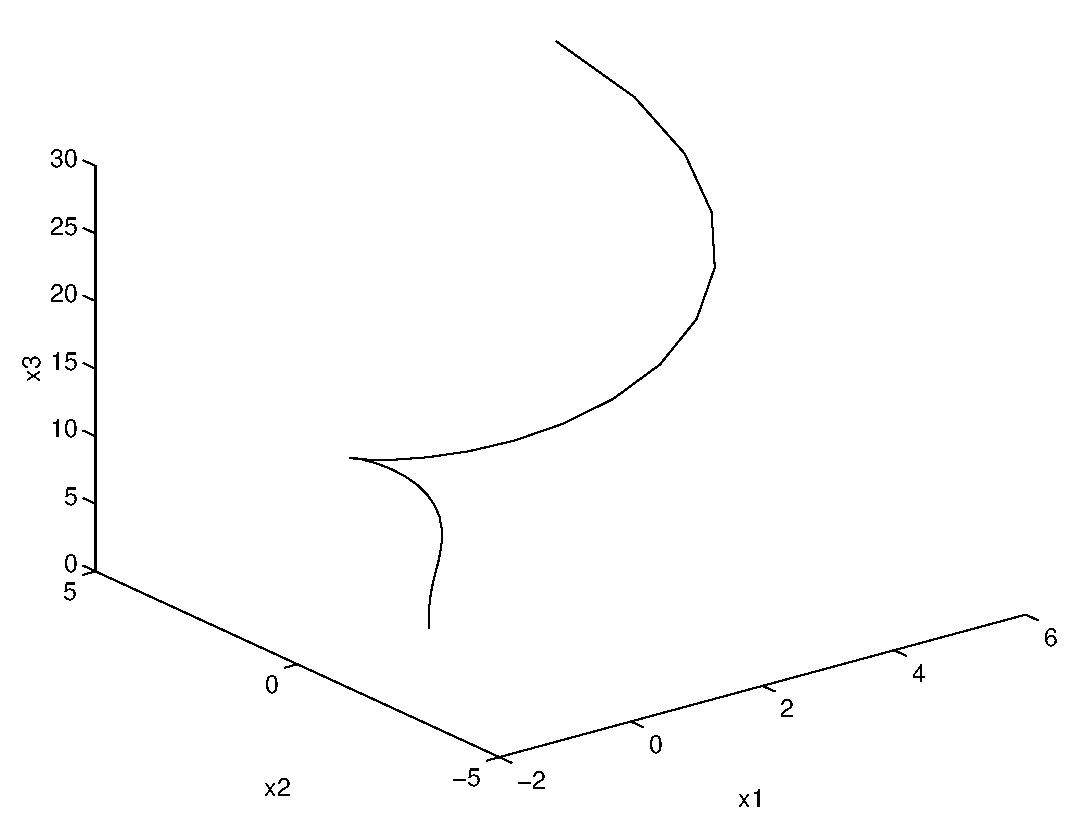
\psfig{file=exfigure/11-4-2a.eps,width=1.35in}
                       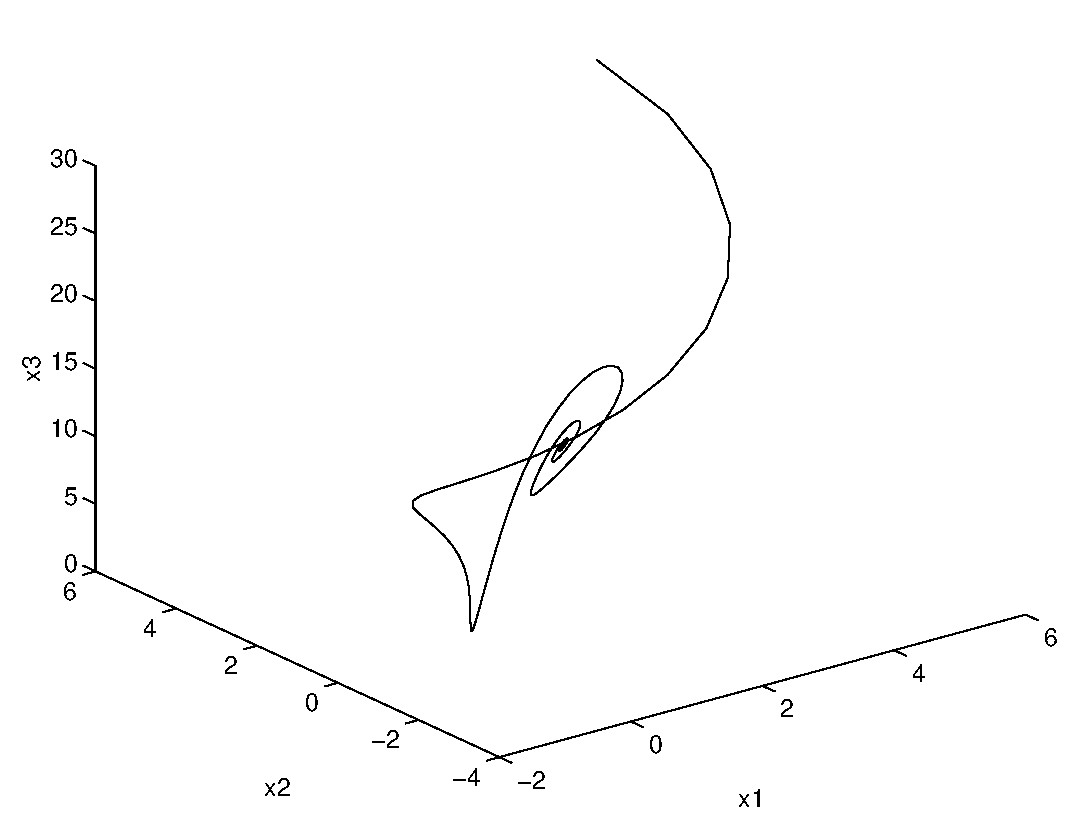
\psfig{file=exfigure/11-4-2b.eps,width=1.35in}
                       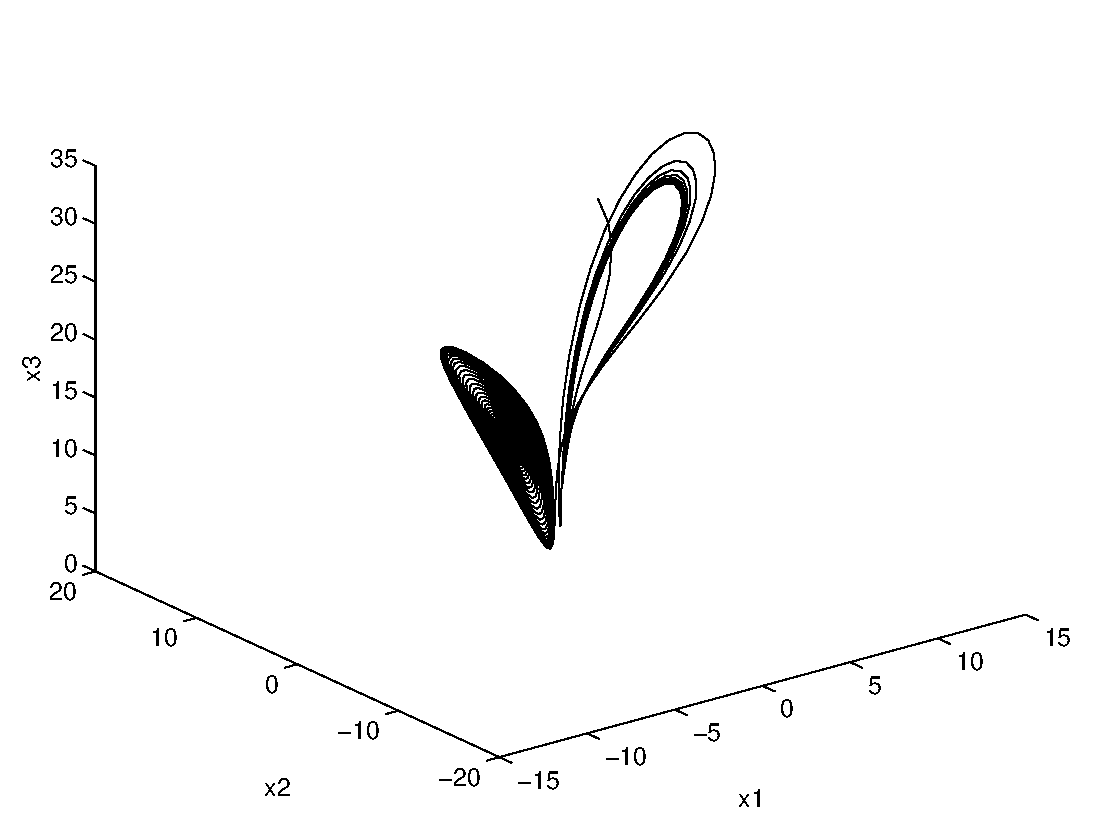
\psfig{file=exfigure/11-4-2c.eps,width=1.35in}
                       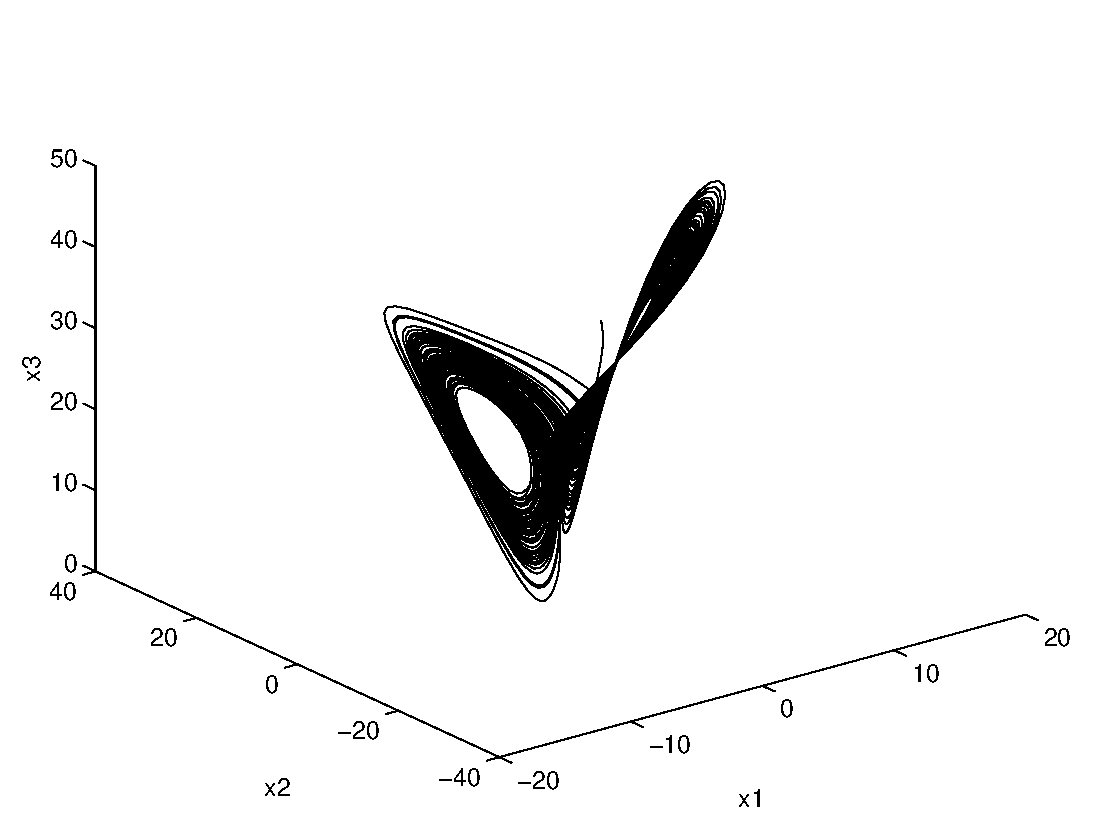
\psfig{file=exfigure/11-4-2d.eps,width=1.35in}}
		\centerline{Figure~\ref{c11.4.2}a\hspace{0.8in}
        	Figure~\ref{c11.4.2}b\hspace{0.8in}Figure~\ref{c11.4.2}c
        	\hspace{0.8in}Figure~\ref{c11.4.2}d}
\end{figure}


\end{solution}
\end{exercise}

\begin{exercise} \label{c11.4.3}
Use {\tt ode45} to analyze the dynamical behavior of a variant of the 
{\em Chua circuit}
\begin{eqnarray*}
  \dot{x} &=& \alpha\left(y-m_0x-\frac{1}{3}m_1x^3\right) \\
  \dot{y} &=& x-y+z \\
  \dot{z} &=& - \beta y.
\end{eqnarray*}
In the computations, fix $\alpha=18$, $\beta=33$, $m_0=-0.2$, and $m_1=0.01$.
You will have to write your own m-file to complete this exercise. 

\begin{solution}

\ans The system has unstable equilibria at $X_1 = (0,0,0)$,
$X_2 = (\sqrt{60},0, -\sqrt{60})$, and $X_3 = (-\sqrt{60},0,\sqrt{60})$.
Figure~\ref{c11.4.3}a shows the behavior of $x$, $y$, and $z$ as $t$
increases.  Figure~\ref{c11.4.3}b shows the graph of the system created
with the {\tt plot3} command.  Figure~\ref{c11.4.3}c shows the same graph
with an overhead view of the $xz$ plane, and with circles indicating the
locations of the equilibria.  In forward time, trajectories oscillate
between circuits around the two nonzero equilibria.

\soln Find the equilibria by finding the points at which $\dot{x} = 0$,
$\dot{y} = 0$, and $\dot{z} = 0$.  Then, compute the general Jacobian
matrix
\[
dJ = \cmatthree{\alpha(-m_0 - m_1x^2)}{\alpha}{0}{1}{-1}{1}{0}{-\beta}{0}
= \cmatthree{-9 - 0.01x^2}{18}{0}{1}{-1}{1}{0}{-33}{0}.
\]
To see that the equilibria are unstable, find the Jacobian matrices at
each equilibrium.  Also note that most trajectories do not converge on
any of the equilibria in forward time.

\begin{figure}[htb]
                       \centerline{%
                       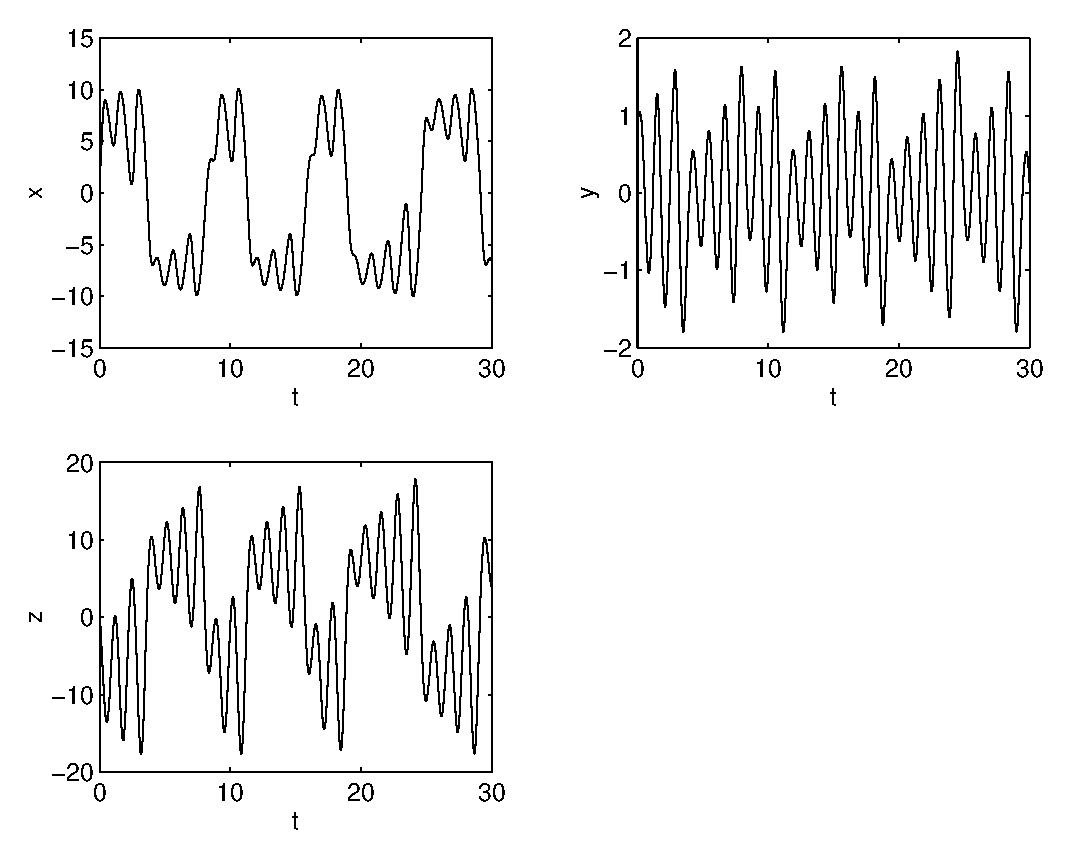
\psfig{file=exfigure/11-4-3a.eps,width=1.35in}
			\hspace{0.5in}
                       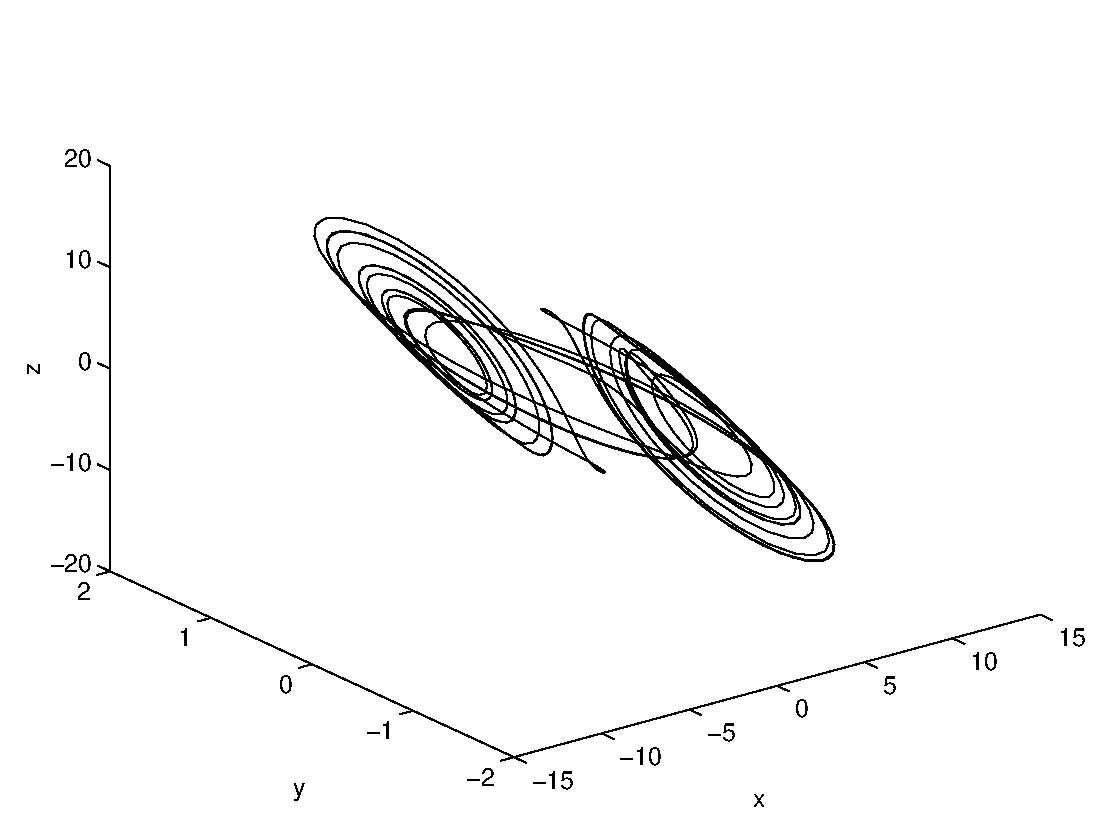
\psfig{file=exfigure/11-4-3b.eps,width=1.35in}
			\hspace{0.3in}
                       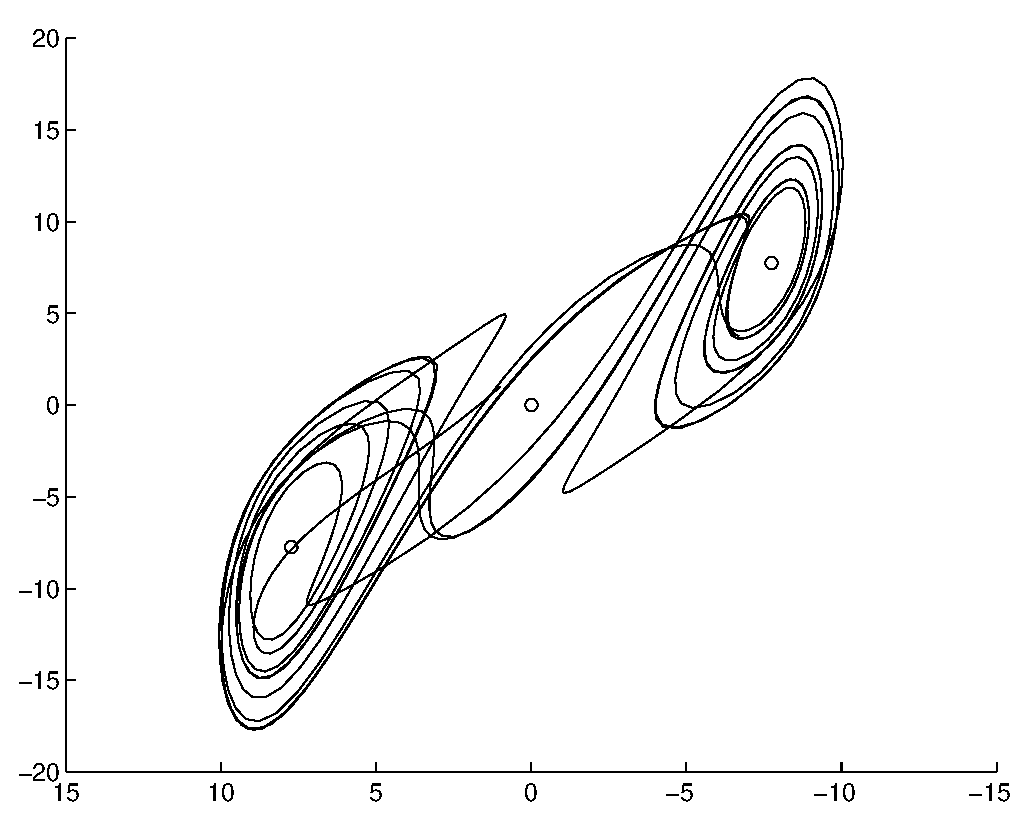
\psfig{file=exfigure/11-4-3c.eps,width=1.35in}}
		\exercapthree{c11.4.3}
\end{figure}


\end{solution}
\end{exercise}

\begin{exercise} \label{c11.4.3a}
Numerically integrate the Lorenz equations \eqref{e:Lorenz} for the standard 
parameter values $\sigma=10$, $\beta=\frac{8}{3}$, $\rho=28$ using the initial 
condition $X_0 =(5.01,5,30)$.  Compare the phase space plot of this solution 
with that of Figure~\ref{fig:lorenz3}.  (You will need to use the same view
point and axis range as was used in that figure.)  Experiment with several 
different choices of initial conditions.

\begin{solution}
Computer experiment.

\end{solution}
\end{exercise}


\noindent In Exercises~\ref{c11.6.1a} -- \ref{c11.6.1h}, determine whether the 
given solution is asymptotic to an equilibrium, a limit cycle, a two-frequency 
torus, exhibits sensitive dependence on initial conditions, or has a limiting 
behavior that has not been described previously.

\begin{exercise}  \label{c11.6.1a}
Solve the system \eqref{e11.6.1a} with initial conditions 
$X_0 = (0.10, 0.20, 0.25)^t$:
\begin{matlabEquation} \label{e11.6.1a}
\begin{array}{rcl} 
\dot{x}_1 & = & 1 - x_1 - x_2^2 \\
\dot{x}_2 & = & -x_2-x_3^2   \\
\dot{x}_3 & = & x_3 +x_1x_2-x_3^3.   \end{array} 
\end{matlabEquation}

\begin{solution}
\ans The solution is asymptotic to an equilibrium.

\soln Solve the system using the m-file:
\begin{verbatim}
function f = f14_6_5(t,x)
f = [1 - x(1) - x(2)*x(2); -x(2) - x(3)*x(3); x(3) + x(1)*x(2) - x(3)^3];
\end{verbatim}

Compute the solution using \Matlab as follows:
\begin{verbatim}
[t,x] = ode45('f14_6_5',[0,40],[0.1, 0.2, 0.25]');
\end{verbatim}

The time series are given in Figure~\ref{c11.6.1a} and show
that each coordinate function is eventually constant.  So the asymptotic
solution is an equilibrium.

\begin{figure}[htb]
     \centerline{%
     \psfig{file=exfigure/figf14_6_2.eps,width=3.5in}}
	\exercap{c11.6.1a}
\end{figure}

\end{solution}
\end{exercise}

\begin{exercise}  \label{c11.6.1d}
Solve the system \eqref{e11.6.1d} with initial conditions 
$X_0 = (0.10, 0.24, 0.14)^t$:
\begin{matlabEquation} \label{e11.6.1d}
\begin{array}{rcl} 
\dot{x}_1 & = &   (x_3 - 1.3)x_1 - 3.5x_2 \\
\dot{x}_2 & = & 3.5x_1 + (x_3-1.3)x_2  \\
\dot{x}_3 & = &
0.6+x_3-\frac{1}{3}x_3^3-(x_1^2+x_2^2)(1+\frac{1}{4}x_3).\end{array}
\end{matlabEquation}

\begin{solution}
\ans The solution is asymptotic to a periodic solution.

\soln Solve the system using the m-file:
\begin{verbatim}
function f = f14_6_6(t,x)
a = 3.5; b = 1.3; c = 0.6; d = 0.25;
f = [(x(3) - b)*x(1) - a*x(2); 
     a*x(1) + (x(3)-b)*x(2); 
     c + x(3) - x(3)^3/3 - (x(1)^2 + x(2)^2)*(1 + d*x(3))];
\end{verbatim}

Compute the solution using \Matlab as follows:
\begin{verbatim}
[t,x] = ode45('f14_6_6',[0,40],[0.10, 0.24, 0.14]');
\end{verbatim}
The time series plot in Figure~\ref{c11.6.1d} shows convergence to a periodic 
solution.  

\begin{figure}[htb]
     \centerline{%
     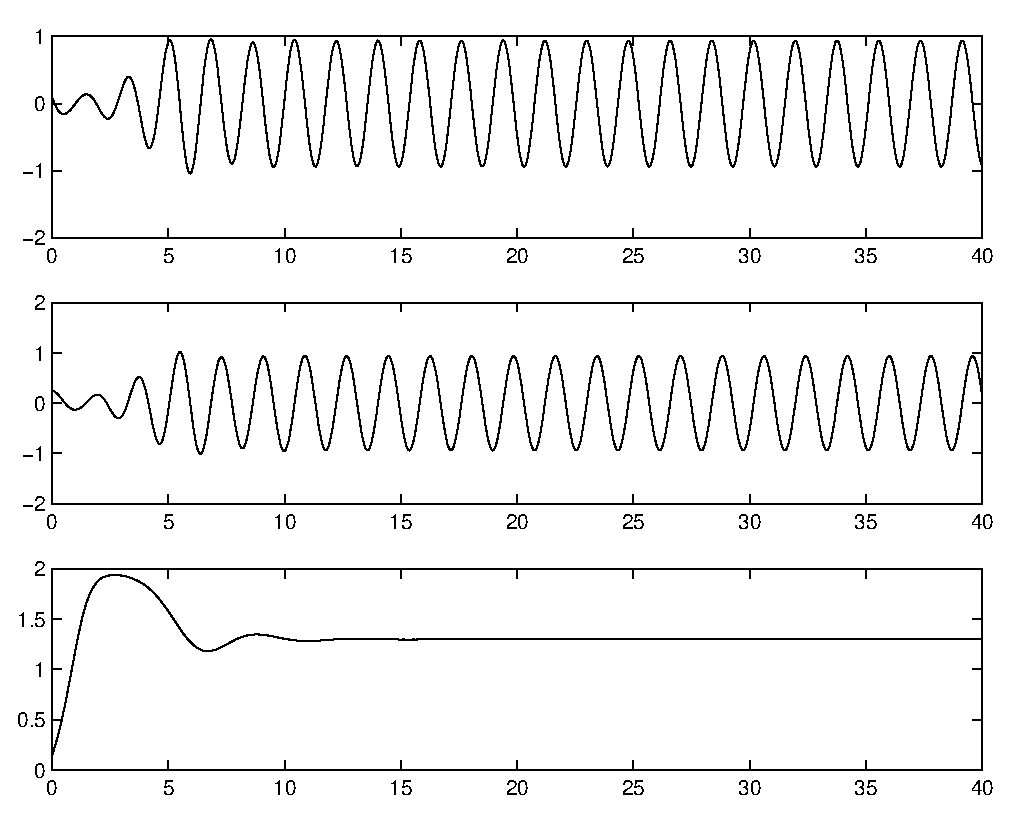
\psfig{file=exfigure/figf14_6_5.eps,width=3.5in}}
	\exercap{c11.6.1d}
\end{figure}

\end{solution}
\end{exercise}

\begin{exercise}  \label{c11.6.1c}
Solve the system \eqref{e11.6.1c} with initial conditions 
$X_0 = (0.10, 0.23, 0.15)^t$:
\begin{matlabEquation} \label{e11.6.1c}
\begin{array}{rcl} 
\dot{x}_1 & = & x_1 - (x_1^2 + 1.5x_2^2 + 0.6x_3^2)x_1 \\
\dot{x}_2 & = & x_2 - (0.6x_1^2 + x_2^2 + 1.5x_3^2)x_2  \\
\dot{x}_3 & = & x_3 - (1.5x_1^2 + 0.6x_2^2 + x_3^2)x_3.   \end{array}. 
\end{matlabEquation}

\begin{solution}
\ans The solution is a new form of asymptotic behavior.

\soln Solve the system  using the m-file:
\begin{verbatim}
function f = f14_6_7(t,x)
a= 1.0; b = 1.5; c = 0.6;
f = [x(1) - (a*x(1)^2 + b*x(2)^2 + c*x(3)^2)*x(1) 
        x(2) - (c*x(1)^2 + a*x(2)^2 + b*x(3)^2)*x(2)
        x(3) - (b*x(1)^2 + c*x(2)^2 + a*x(3)^2)*x(3)];
\end{verbatim}
Compute the solution using \Matlab as follows:
\begin{verbatim}
[t,x] = ode45('f14_6_7',[0,1000],[0.10, 0.23, 0.15]');
\end{verbatim}

The time series in Figure~\ref{c11.6.1c}a never settle down but approach in 
order three separate
equilibria.  The solution is asymptotic to a cycle of heteroclinic
trajectories and is a new form of asymptotic behavior.  The three 
dimensional plot of the asymptotic solution is obtained by typing
\begin{verbatim}
size(t)
\end{verbatim}
obtaining
\begin{verbatim}
ans =
        2749           1
\end{verbatim}
and then typing
\begin{verbatim}
s = 500:1:2749;
plot3(x(s,1),x(s,2),x(s,3))
\end{verbatim}
The cycle of heteroclinic orbits is shown in Figure~\ref{c11.6.1c}b.

\begin{figure}[htb]
     \centerline{%
     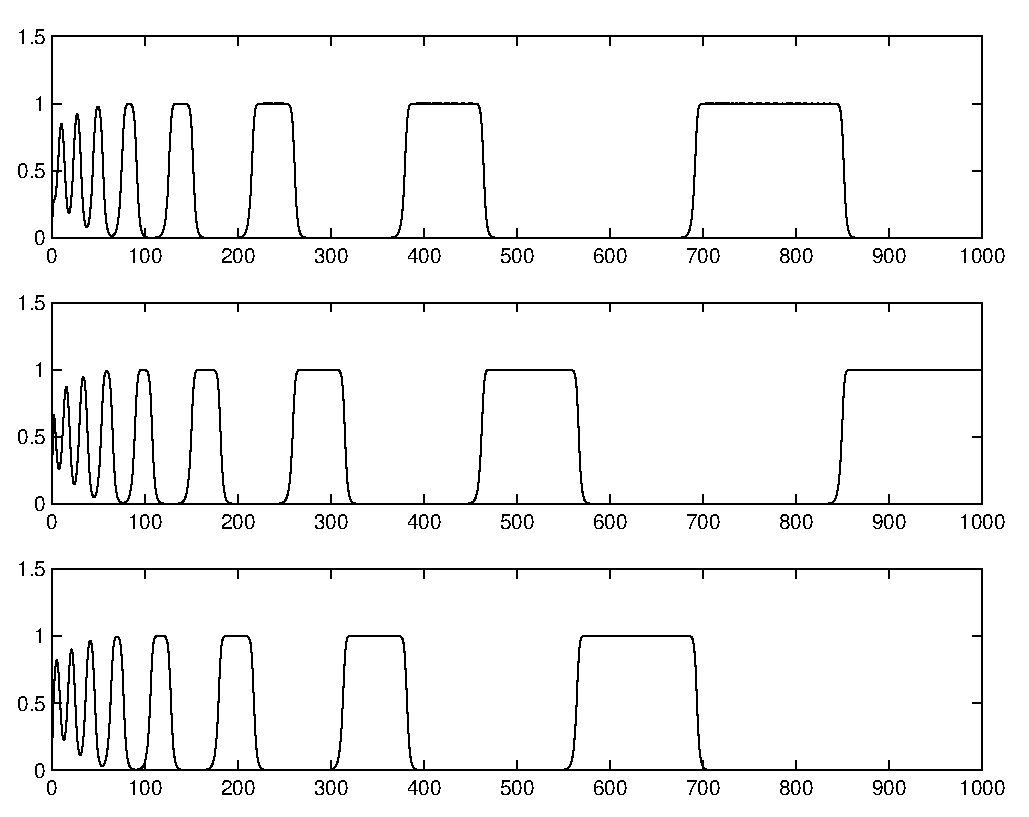
\psfig{file=exfigure/figf14_6_4.eps,width=2.7in}
     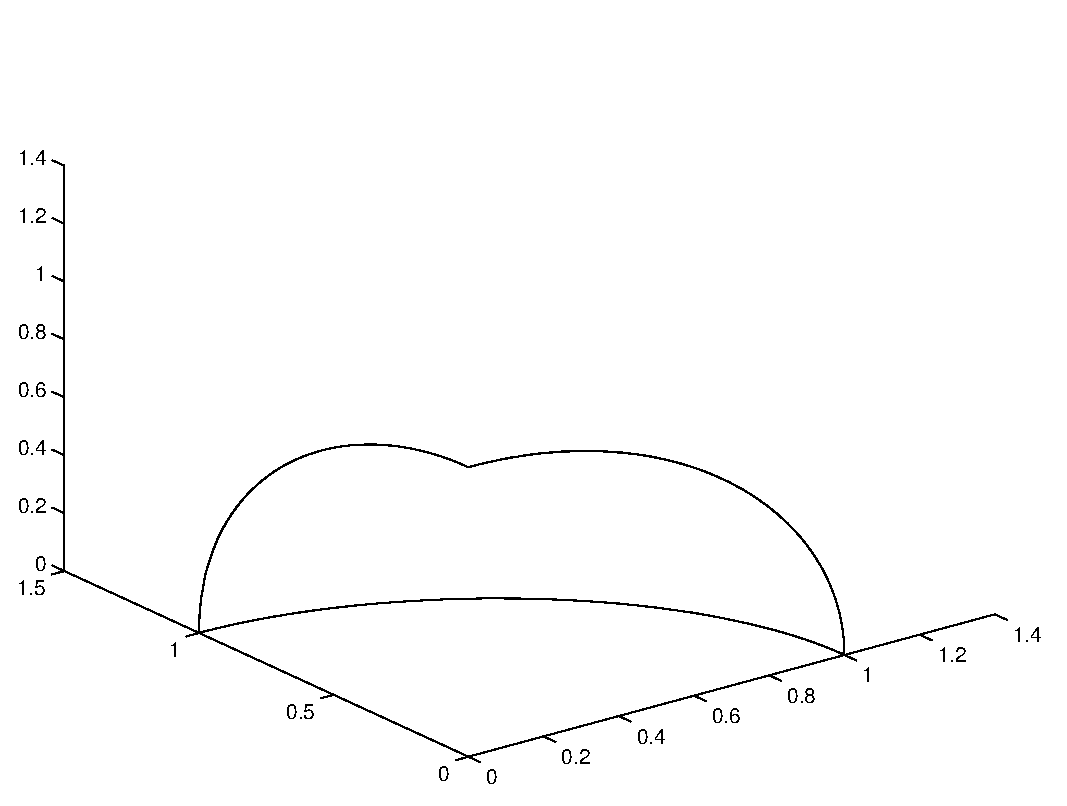
\psfig{file=exfigure/figf14_6_4a.eps,width=2.7in}}
	\exercaptwo{c11.6.1c}
\end{figure}

\end{solution}
\end{exercise}

\begin{exercise}  \label{c11.6.1b}
Solve the system \eqref{e11.6.1b} with initial conditions 
$X_0 = (0.10, 0.23, 0.15)^t$:
\begin{matlabEquation} \label{e11.6.1b}
\begin{array}{rcl} 
\dot{x}_1 & = & x_1 - (x_1^2 + 0.5x_2^2 + 0.7x_3^2)x_1 \\
\dot{x}_2 & = & x_2 - (0.7x_1^2 + x_2^2 + 0.5x_3^2)x_2  \\
\dot{x}_3 & = & x_3 - (0.5x_1^2 + 0.7x_2^2 + x_3^2)x_3.   \end{array}
\end{matlabEquation}

\begin{solution}
\ans The solution is asymptotic to an equilibrium.

\soln Solve the system using the m-file:
\begin{verbatim}
function f = f14_6_8(t,x)
a= 1.0; b = 0.5; c = 0.7;
f = [x(1) - (a*x(1)^2 + b*x(2)^2 + c*x(3)^2)*x(1) 
        x(2) - (c*x(1)^2 + a*x(2)^2 + b*x(3)^2)*x(2)
        x(3) - (b*x(1)^2 + c*x(2)^2 + a*x(3)^2)*x(3)];
\end{verbatim}
Compute the solution using \Matlab as follows:
\begin{verbatim}
[t,x] = ode45('f14_6_8',[0,100],[0.10, 0.23, 0.15]');
\end{verbatim}
The time series are given in Figure~\ref{c11.6.1b} and show
that each coordinate function is eventually constant.  So the asymptotic
solution is an equilibrium.

\begin{figure}[htb]
     \centerline{%
     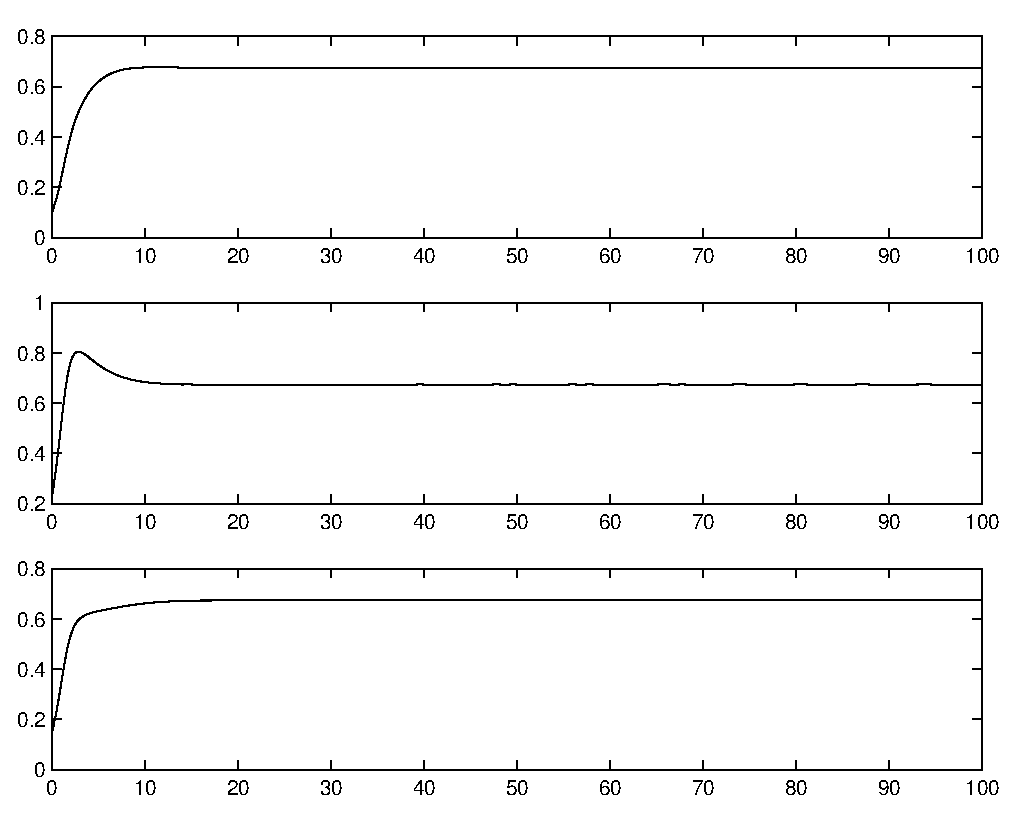
\psfig{file=exfigure/figf14_6_3.eps,width=3.5in}}
	\exercap{c11.6.1b}
\end{figure}

\end{solution}
\end{exercise}

\begin{exercise}  \label{c11.6.1e}             
Solve the system \eqref{e11.6.1e} with initial conditions 
$X_0 = (0.10, 0.11, 0.15)^t$:
\begin{matlabEquation} \label{e11.6.1e}
\begin{array}{rcl} 
\dot{x}_1 & = & -x_2-x_3  \\
\dot{x}_2 & = &  x_1 + 0.2x_2 \\
\dot{x}_3 & = & 0.2 + x_3(x_1 - 5.7). \end{array}
\end{matlabEquation}

\begin{solution}
\ans The asymptotic dynamics of this solution is chaotic.

\soln Solve the system using the m-file:
\begin{verbatim}
function f = f14_6_9(t,x)
a = 5.7; b = 0.2; c = 0.2;
f = [-x(2)-x(3); 
     x(1) + b*x(2); 
     c + x(3)*(x(1)-a)];
\end{verbatim}

Compute the solution using \Matlab as follows:
\begin{verbatim}
[t,x] = ode45('f14_6_9',[0,400],[0.10, 0.11, 0.15]');
\end{verbatim}
This integration takes awhile.  The three dimensional plot of the
solution is given in Figure~\ref{c11.6.1e}.  Note the complicated behavior
reminiscent of the Lorenz equations.  The asymptotic dynamics of this
solution is chaotic.  Sensitive dependence on initial conditions can be
checked.

\begin{figure}[htb]
     \centerline{%
     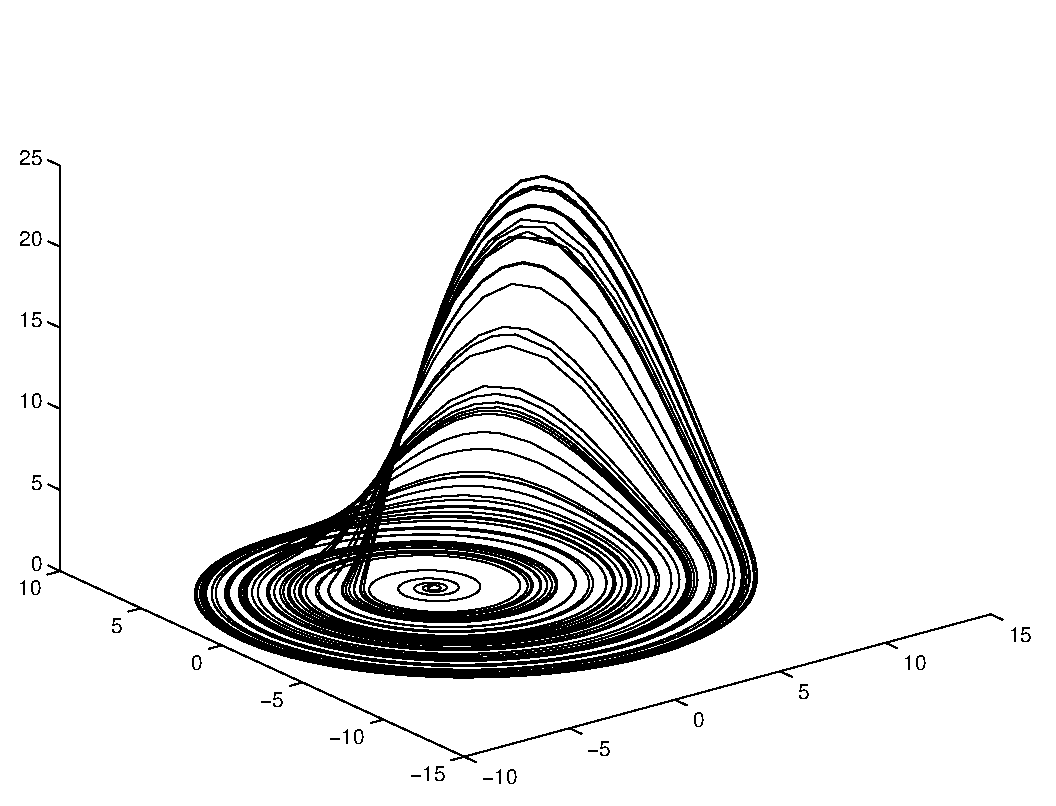
\psfig{file=exfigure/figf14_6_6.eps,width=3.0in}}
	\exercap{c11.6.1e}
\end{figure} 

\end{solution}
\end{exercise}

\begin{exercise}  \label{c11.6.1g} 
Solve the system \eqref{e11.6.1g} with initial conditions 
$X_0 = (0.1,0.2, -0.2)^t$:
\begin{matlabEquation} \label{e11.6.1g}
\begin{array}{rcl} 
\dot{x}_1 & = & 0.65 + x_1 - x_1^{10} - (x_3^2 + x_2^2)(1 + 0.25x_1)  \\
\dot{x}_2 & = & 3.5x_3 + (x_1 - 0.7)x_2  \\
\dot{x}_3 & = & (x_1 - 0.7)x_3 - 3.5x_2.
\end{array}
\end{matlabEquation}

\begin{solution}
\ans The solution is asymptotic to a two-frequency torus.

\soln Solve the system using the m-file:
\begin{verbatim}
function f = f14_6_10(t,x)
f = [0.65 + x(1) - x(1)^(10) - (x(3)^2+x(2)^2)*(1+0.25*x(1)); 
     3.5*x(3) + (x(1)-0.7)*x(2); 
     (x(1)-0.7)*x(3) - 3.5*x(2)];
\end{verbatim}

Compute the solution using \Matlab as follows:
\begin{verbatim}
[t,x] = ode45('f14_6_10',[0,40],[0.10, 0.2, -0.2]');
\end{verbatim}
The phase space plot in Figure~\ref{c11.6.1g}a shows asymptotic convergence to
a two-frequency torus.

Note that the $x_1$ times series in Figure~\ref{c11.6.1g}b 
suggests time periodic behavior, while the $x_2$ and $x_3$ time series 
show more clearly two-frequency motion.  Compare this comment with the
three-dimensional phase space plot.

\begin{figure}[htb]
     \centerline{%
     \psfig{file=exfigure/figf14_6_7.eps,width=2.7in}
     \psfig{file=exfigure/figf14_6_7a.eps,width=2.7in}}
	\exercaptwo{c11.6.1g}
\end{figure} 


\end{solution}
\end{exercise}

\begin{exercise}  \label{c11.6.1f}
Solve the system \eqref{e11.6.1f} with initial conditions 
$X_0 = (2.0, 0.5, 1.0)^t$:
\begin{matlabEquation} \label{e11.6.1f}
\begin{array}{rcl} 
\dot{x}_1 & = & -x_2-x_3  \\
\dot{x}_2 & = &  x_1 + 0.2x_2 \\
\dot{x}_3 & = & 0.2 + x_3(x_1 - 1). \end{array}
\end{matlabEquation}

\begin{solution}
\ans The solution is asymptotic to a periodic solution.

\soln Solve the system using the m-file:
\begin{verbatim}
function f = f14_6_11(t,x)
a = 1; b = 0.2; c = 0.2;
f = [-x(2)-x(3); 
     x(1) + b*x(2); 
     c + x(3)*(x(1)-a)];
\end{verbatim}

Compute the solution using \Matlab as follows:
\begin{verbatim}
[t,x] = ode45('f14_6_11',[0,80],[2.0, 0.5, 1.0]');
\end{verbatim}
The time series plot in Figure~\ref{c11.6.1f} shows convergence to a periodic solution.  

\begin{figure}[htb]
     \centerline{%
     \psfig{file=exfigure/figf14_6_8.eps,width=3.0in}}
	\exercap{c11.6.1f}
\end{figure} 

\end{solution}
\end{exercise}

\begin{exercise}  \label{c11.6.1h} 
Solve the system \eqref{e11.6.1h} with initial conditions 
$X_0 = (3.0084, 3.0983, 2.7673)^t$: 
\begin{matlabEquation} \label{e11.6.1h}
\begin{array}{rcl} 
\dot{x}_1 & = &  -1.5x_1 + (x_3-0.2)x_2 \\
\dot{x}_2 & = &  -1.5x_2 + x_1x_3\\
\dot{x}_3 & = &  1 - x_1x_2.
\end{array}
\end{matlabEquation}

\begin{solution}
\ans The solution is chaotic.

\soln Solve the system using the m-file:
\begin{verbatim}
function f = f14_6_12(t,x)
a = 1.5; b = 0.2; c = 1;
f = [    -a*x(1) + (x(3)-b)*x(2);
-a*x(2)+x(1)*x(3);   
     c - x(1)*x(2)];
\end{verbatim}

Compute the solution using \Matlab as follows:
\begin{verbatim}
[t,x] = ode45('f14_6_12',[0,200],[3.0084 3.0983 2.7673]');
\end{verbatim}
The time series never settle down (see Figure~\ref{c11.6.1h}a) and it is 
possible to test for sensitive dependence on initial conditions. 
The three-dimensional phase space plot in Figure~\ref{c11.6.1h}b looks like 
a very thin Lorenz attractor.  

\begin{figure}[htb]
     \centerline{%
     \psfig{file=exfigure/figf14_6_9.eps,width=2.7in}
     \psfig{file=exfigure/figf14_6_9a.eps,width=2.7in}}
	\exercaptwo{c11.6.1h}
\end{figure} 

















\end{solution}
\end{exercise}
\end{document}
